\documentclass{article} % For LaTeX2e
\usepackage[utf8x]{inputenc}
\usepackage[T1]{fontenc}
\usepackage{nips11submit_e,times}
\usepackage{natbib}
\usepackage{amsmath}
\usepackage{graphicx}
\usepackage{verbatim}
%\documentstyle[nips10submit_09,times,art10]{article} % For LaTeX 2.09


\title{A Common GPU n-dimensions array}


\author{
Frédéric Bastien, Arnaud Bergeron, Pascal Vincent and Yoshua Bengio \\
D\'epartement d'Informatique et de Recherche Op\'erationnelle\\
Universit\'e de Montr\'eal\\
Montr\'eal, Canada \\
\texttt{\{bastienf, bergearn, vincentp, bengioy\}@iro.umontreal.ca} \\
}

% The \author macro works with any number of authors. There are two commands
% used to separate the names and addresses of multiple authors: \And and \AND.
%
% Using \And between authors leaves it to \LaTeX{} to determine where to break
% the lines. Using \AND forces a linebreak at that point. So, if \LaTeX{}
% puts 3 of 4 authors names on the first line, and the last on the second
% line, try using \AND instead of \And before the third author name.

\newcommand{\fix}{\marginpar{FIX}}
\newcommand{\new}{\marginpar{NEW}}

\nipsfinalcopy % Uncomment for camera-ready version

\begin{document}


\maketitle

\begin{abstract}
Currently there are multiple incompatible array/matrix/n-dimensional object implementations
that exist for GPUs. This hinders sharing of GPU code and causes
duplicate development work. This paper proposes and presents a
first version of a common GPU n-dimensional
array(tensor) named ~\citep{GpuNdArray} that works with both CUDA and OpenCL. 
It will be usable in python, C++ and possibly others languages.
\end{abstract}

\section{Introduction}
Currently there are at least 4 different GPU array implementations in
python: CudaNdarray(Theano)~\citep{bergstra+al:2010-scipy},
GPUArray(PyCUDA)~\citep{kloeckner_pycuda_2009},
GPUArray(PyOpenCL)~\citep{kloeckner_pycuda_2009} and
CUDAMatrix(cudamat)~\citep{cudamat-TR2009}. There are also other
implementations like Trust~\citep{Thrust} in C++. One problem is that they are
incompatible with each other. Each of them implements a different
subset of the features that Numpy~\citep{numpy-2007} provides on the
CPU, namely a tensor object (arbitrary-dimensional array) with support
for \emph{strides}~\footnote{
\emph{Strides} are a way to specify for each dimensions in an an n-dimentional object a subrange and the number of elements to skip when going
to the next element. E.g. This allows
to operate on a view that represents only odd, even, every third row, etc$\ldots$ of
a matrix. This avoids copying data and lowers the memory usage and memory
access. The part to view in each dimensions is specified as a range of elements, with a
step between each elements. This is represented with slice with a start(included) index, an
end(excluded) index and a step.
}
 and \emph{broadcasting}~\footnote{
\emph{Broadcasting} is a generalization on tensors of the convention and mechanism that allows e.g. adding a
vector to all rows or columns of a matrix. Not all existing gpu array implementations
support this very useful construct. It is however easy to add when we have
stride support. As Numpy has it, we would like to keep it.}.  Some implementations
support only vectors or matrices, some support only \emph{float32},
only contiguous memory layout, etc$\ldots$ None of them targets both
CUDA and OpenCL.

The goal is to have a common GPU object that we hope will be used by everybody with the following conditions:

\begin{itemize}
\item Make a n-dimensional array on the gpu that supports strides and broadcasting
\item Don't make development harder with this n-dimensional array. 
\item Make the python interface similar to numpy.ndarray
  \begin{itemize}
  \item Easier to attract other people from python community
  \end{itemize}
\item Have the base object in C to allow collaboration with other non-python projects.
  \begin{itemize}
  \item We want people from C, C++, ruby, R, etc... to all use the same base Gpu ndarray.
  \end{itemize}
\item Be compatible with CUDA and OpenCL
\end{itemize}

We believe that for a common GPU object, we need an n-dimensional
array. The motivation is that forcing users to use an object that
supports only 1 or 2 dimensions adds complexity when dealing with algorithms that have natively more than 2 dimensions.
We don't think that this complexity should be dealt with by each user and 
having a base object that supports n-dimensions, removes
this complexity.

We believe that there are several reasons why there has not yet been a common GPU implementation fulfilling our objectives.
One may be that such a general tensor implementation on GPU is hard and time consuming to get right and efficient.

From the developer's point of view, sometimes it is useful to support general strides in inputs and sometimes not.
In the case where the developer does not want general strides in inputs, we think
that calling a function to assert/convert the inputs to the desired layout is not too complicated or time consuming.
Especially when those functions are provided. For example, if a
developer writes a kernel that only supports C-order inputs, he could
just call a function on his inputs to convert each one to a C layout
and then proceed as usual.

\begin{comment}
Many times, the input layout chosen by the developer of a function
will lead to better memory access pattern than a random memory
layout. So it is not trivial to say that generalizing the
implementation to support general memory layout will lead to
significant performance gain. 
\end{comment}

A second reason why people didn't implement all those features is
that having more dimensions and having general strides take more
computation for indexing. This can lead to slower code. Lets examine the example of the addition of 2 tensors of 10 dimensions.
In serial code, having more dimensions just adds more imbricated loops.  
If you loop over the dimensions on the right order (according to the layout) and the inner loop is big enough, having more loops will not make much of a difference.
In parallel code, it is much harder to make the indexing computations not overshadow the actual computations. 
CUDA can provide only up to 5 implicit loops. So all extra dimensions require
additional indexing computation. Also, if the size of those dimensions
are not suited to the GPU, this can lead to lower performance.

Optimizations are possible for computing the indexing, like
collapsing some dimensions on the cpu and implicitly using a kernel
that uses fewer dimensions. The trick lies in knowing which 
dimensions you can collapse for which function and inputs. This is
implemented for elemwise operations as discussed in the ``Current
implementation'' section.

We think that if we provide such optimized functions for element wise and
reduction operations, we will cover enough cases where the conversion from
one memory layout to another can be combined with computations. This
can still impact the performance due to coalescing constraints, but we
don't expect that to be significant most of the time.

\begin{comment}
The lack of a common GPU tensor create many problems. Here is a few:
\begin{itemize}
  \item Duplicate work
  \item Harder to port/reuse code
  \item Harder to find/distribute code
  \item Divides development work
\end{itemize}

All those problem are aggravated by the fact that GPU code is
harder/slower to do correctly and fast than serial CPU code.
\end{comment}

\section{Existing Implementation}
\subsection{Theano(CudaNdarray)}
Theano is the system that provides the closest approximation of a GPU tensor. According to its web site Theano~\citep{bergstra+al:2010-scipy} is:
``a Python library that allows you to define, optimize, and evaluate mathematical expressions involving multi-dimensional arrays efficiently''.

It implements a GPU tensor with strides and broadcasting, but supports only single precision floating point and CUDA. Also, the strides information are stored differently than numpy. Theano stores the number of elements to skip to access the next element and numpy stores the number of bytes to skip.

\subsection{PyCUDA/PyOpenCL(GPUArray)}
PyCUDA~\citep{kloeckner_pycuda_2009} and PyOpenCL~\citep{kloeckner_pycuda_2009} are python wrappers around CUDA and OpenCL respectively. In addition to wrapping their respective library, they do automatic memory management, add a GPUarray object and some abstraction for compilation. They also automatically translates errors to python exceptions.

Their GPU array objects are limited to contiguous memory regions. They add shape properties to allow using this contiguous memory region as n-dimensional array. They don't support strides or broadcasting, but they support many data types. Both wrappers can be used together in the same python script.

\subsection{CUDAMat}
The CUDAMat~\citep{cudamat-TR2009} web site describes itself with: ``The aim of the cudamat project is to make it easy to perform basic matrix calculations on CUDA-enabled GPUs from Python. cudamat provides a Python matrix class that performs calculations on a GPU.''

So we clearly see that it support only CUDA and matrix. If we look deeper we see that it doesn't support strides and supports only single precision floating point. Broadcasting is supported via a function and not via the usual numpy syntax.

\subsection{Gnumpy}
Gnumpy~\citep{gnumpy-TR2010} is built on top of cudamat. It allows to work with n-dimensional arrays when they are contiguous in memory. So, no support for strides. It also adds support for the boolean type by using 1.0 and 0.0 in floating point to represent true and false, respectively. It also supports broadcasting via numpy syntax.

\subsection{Trust}
Trust~\citep{Thrust} is a C++ template library. It provides a vector object for cuda. It supports all data types.  Also, as it supports only 1 dimension, there are no means of broadcasting nor strides.

\subsection{Summary}
We see clearly that none of those implementations offer all of what we want for a common GPU tensor. As the Theano implementation supports strides and that it is easier to add other types than to add strides support, we used much of its code as a starting point for our implementation. Theano also implemented some optimizations to lower the performance loss of having more dimensions.

\section{Current implementation}

We currently have all the code implemented and working for CUDA.
OpenCL is partially implemented and some adjustments remain to be done.

\subsection{Functionality}

The current code can allocate arrays, transfer data to and from the CPU, create view of that data and run elemwise kernels on that data.  In order to support multiple APIs we have created a list of utility functions that are to be implemented for each API and the rest of the code is shared.

The language independent parts take care of indexing, making views, and provide an API that is very similar to numpy.  This is the part that supports any (valid) combination of dimensions and strides.  \emph{(mabye) Most importantly, the element-wise kernels and dimension collapsing optimizations are device-independent and can be reused between APIs.}

We are still missing some items before we reach full numpy compatibility, most importantly reductions, setting a part of the array via assignation and reshaping.

\begin{comment}
fct implemented language dependent
cuda
malloc/free
memcopy
memset
from cpu to gpu
from gpu to cpu

gpu agnos:
sub tensor
deepcopy
view
zeros
empty

probably gpu agnos, not sure:
elemwise
elemwise dimensions collapsing


todo:
assignation
reshape
n dimensional tranpose
dot22,gemm
reduce along all dimensions, along one axis or a list of dimensions
reduce dimensions collapsing
\end{comment}

\subsection{Elemwise dimensions collapsing}
To lower the indexing computation cost with more dimensions, we can
try to \emph{collapse} consecutive dimensions for the purpose of doing
element-wise computation. For example if we want to add 2 tensors of
10 dimensions and that both of them are c contiguous, we can use the
same gpu function as for tensor of 1 dimension. This will give the
same results but with fewer index calculations.

We can extend this to more case. If we still want to add 2 tensors of
2 dimensions, but one inputs is strided on the outermost dimensions,
we don't want to pay the indexing computation for 10 dimensions. In
this case, we can collapse all dimensions together except the outer
most dimensions. This will result in paying indexing of a matrix, not
for 10 dimensions.

\section{Benchmarks}

In order to measure the overhead of multiple dimensions and strides in comparison to existing implementations, we compared some elementwise kernels generated with PyCUDA to some generated using our algorithm (including dimension collapsing and strides data).
The timings shown below do not include any transfer time or allocation of output array.
They were made on a GeForce GTX 580.

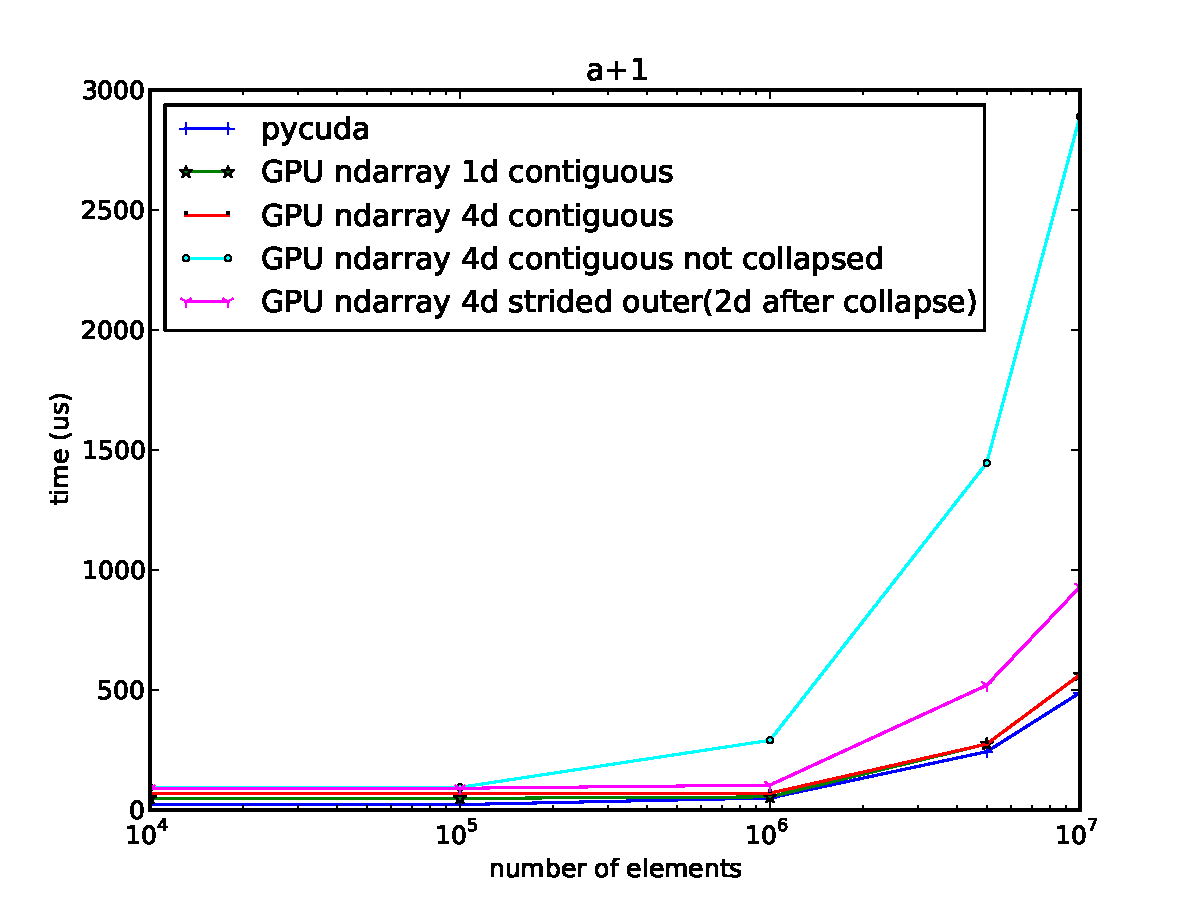
\includegraphics[width=0.5\textwidth]{ap1_no_alloc}
%%\includegraphics[width=0.5\textwidth]{apb_no_alloc}
%%\includegraphics[width=0.5\textwidth]{2ap3b_no_alloc}
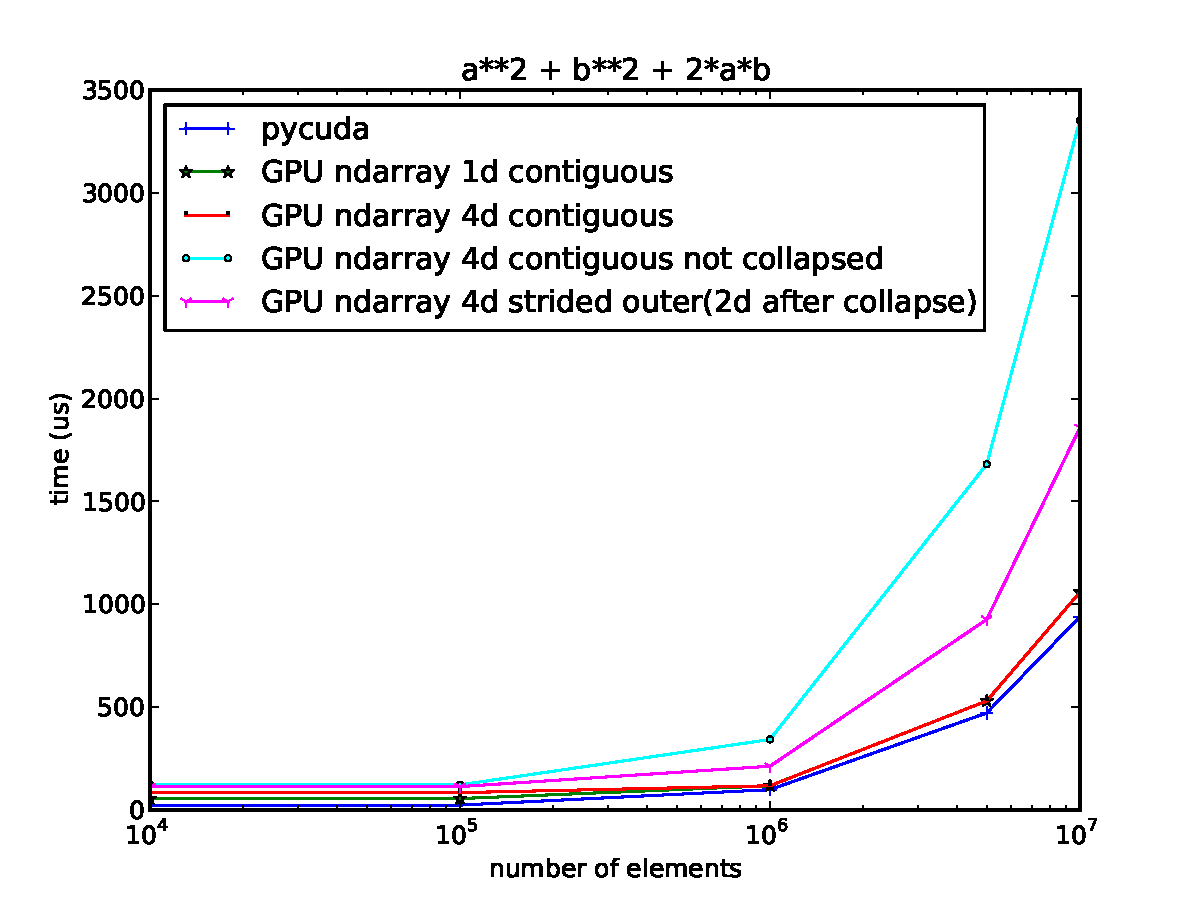
\includegraphics[width=0.5\textwidth]{a2pb2p2ab_no_alloc}

We can conclude from these benchmarks that we have a bigger base cost that PyCUDA.
Although it is interesting to note that the strides code does not add any significant overhead to the computations.TODO: TRUE/FALSE?!?!?

\section{Future Plans}

We plan to continue lowering the elemwise overhead vs PyCUDA. To make
it all functionality working with OpenCL while maximixing the code
reuse. We also plan to implement reduction operation and to contact
people from the C/C++ community to have a good interface available in
that language.

As Theano authors are part of this project, it will get used in a futur Theano version. PyCUDA/PyOpenCL author have started a branch to use this new object.

\section{Conclusion}

%\subsection{Margins in LaTeX}
% 
%Most of the margin problems come from figures positioned by hand using
%\verb+\special+ or other commands. We suggest using the command
%\verb+\includegraphics+
%from the graphicx package. Always specify the figure width as a multiple of
%the line width as in the example below using .eps graphics
%\begin{verbatim}
%   \usepackage[dvips]{graphicx} ... 
%   \includegraphics[width=0.8\linewidth]{myfile.eps} 
%\end{verbatim}
%or % Apr 2009 addition
%\begin{verbatim}
%   \usepackage[pdftex]{graphicx} ... 
%   \includegraphics[width=0.8\linewidth]{myfile.pdf} 
%\end{verbatim}
%for .pdf graphics. 
%See section 4.4 in the graphics bundle documentation (http://www.ctan.org/tex-archive/macros/latex/required/graphics/grfguide.ps) 
% 
%A number of width problems arise when LaTeX cannot properly hyphenate a
%line. Please give LaTeX hyphenation hints using the \verb+\-+ command.


\subsubsection*{Acknowledgments}

We want to thanks James Bergstra. We used some of his code as the first version of some functionality currently implemented. We would also like to acknowledge Compute Canada, RQCHP, NSERC, and Canada Research Chairs for providing fonds or access to compute resources.


\bibliography{strings,strings-shorter,ml,aigaion-shorter}
\bibliographystyle{plain}

\end{document}
